% SIAM Shared Information Template
% This is information that is shared between the main document and any
% supplement. If no supplement is required, then this information can
% be included directly in the main document.
Motivation for developing an alternative method stems from the ESSEX (Equipping Sparse Solvers for Exascale) project \cite{ESSEX}
 where we investigate into solving large eigen-value problems from quantum mechanics field. In this context having a robust iterative solver was inevitable, due to the poor condition number of the matrices that appear in this field. Kaczmarz (\KACZ) solver was found to be satisfactory but parallelizing this solver was deemed challenging because of the loop-carried dependencies in the kernel. Previous work on parallelizing the \KACZ kernel used \MCfull (\MC) \cite{feast_mc} but it was soon found that the kernels do not scale efficiently with this approach.

  \begin{figure}[thbp]
  	\centering
  	\subfloat[$\alpha$ effect]{\label{fig:motivation_a}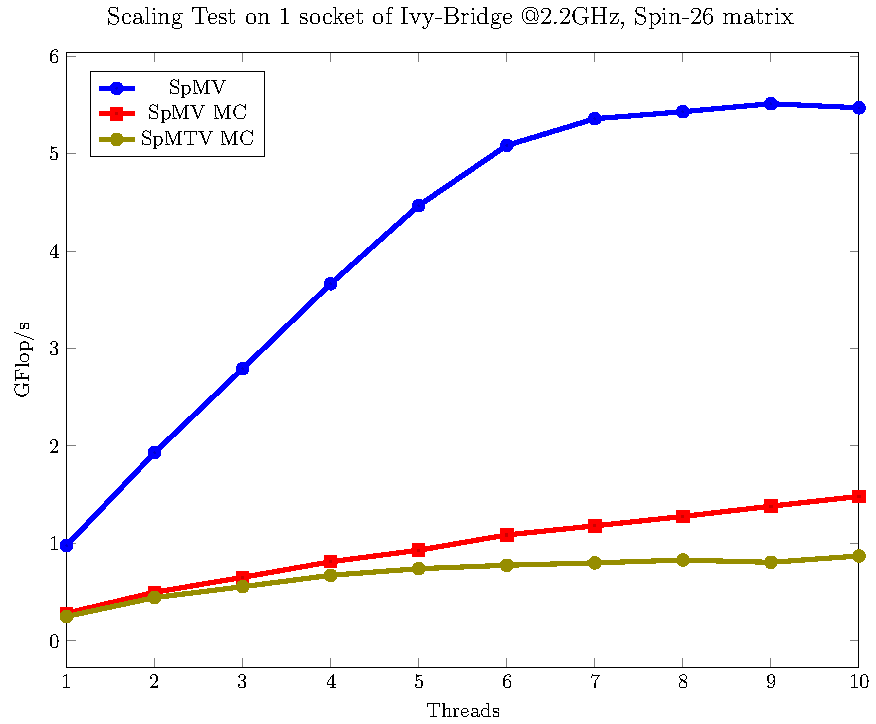
\includegraphics[width=0.45\textwidth, height=0.22\textheight]{pics/motivation/motivation_1}}
  	\hspace{1em}
  	\subfloat[Data Traffic]{\label{fig:motivation_b}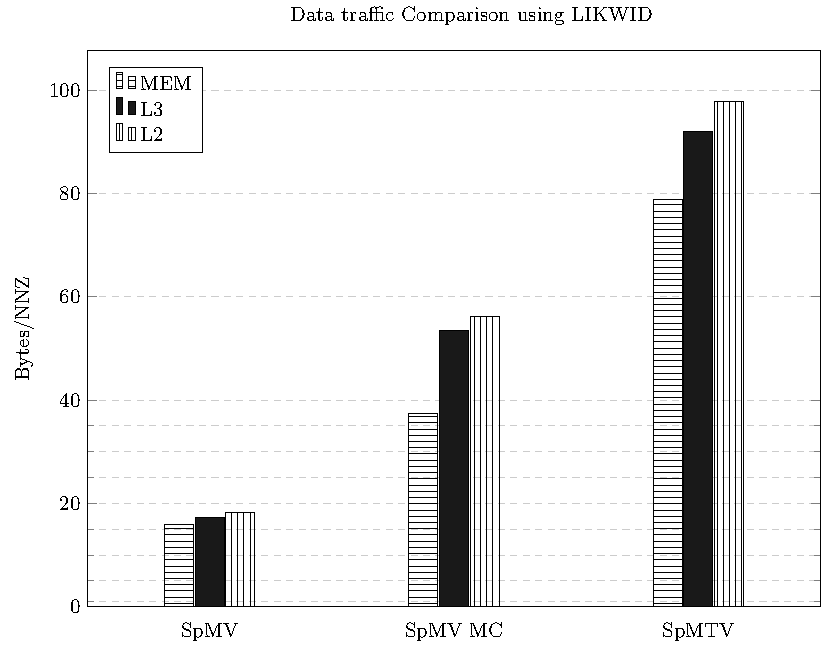
\includegraphics[width=0.45\textwidth, height=0.22\textheight]{pics/motivation/motivation_3}}
  	
  %	\subfloat[False sharing]{\label{fig:motivation_c}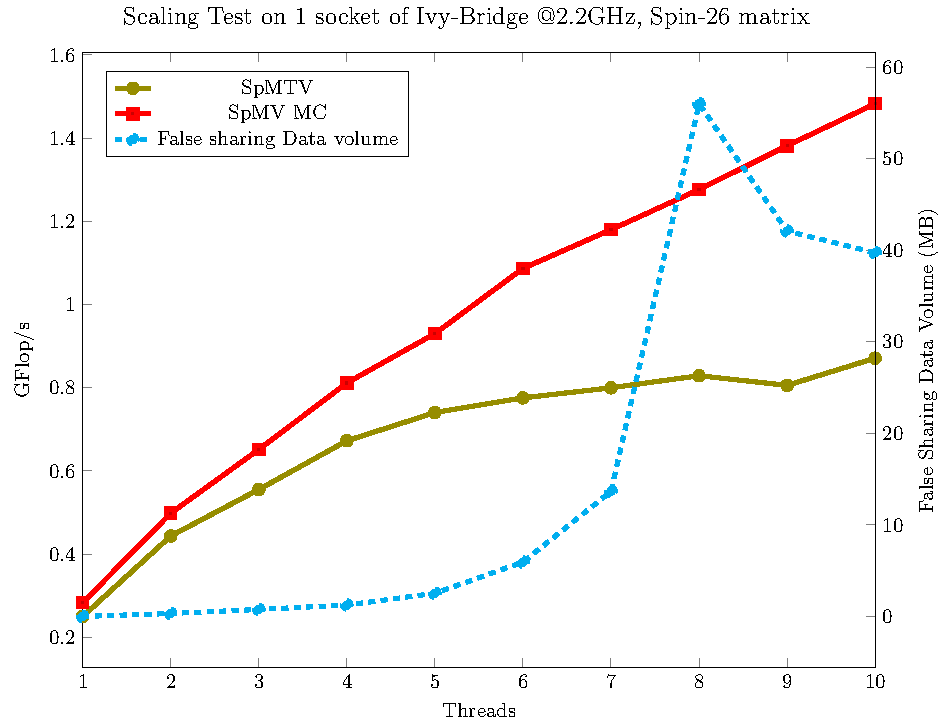
\includegraphics[width=0.45\textwidth, height=0.22\textheight]{pics/motivation/motivation_2}}
  %	\hspace{1em}
  %	\subfloat[Barrier effect]{\label{fig:motivation_d}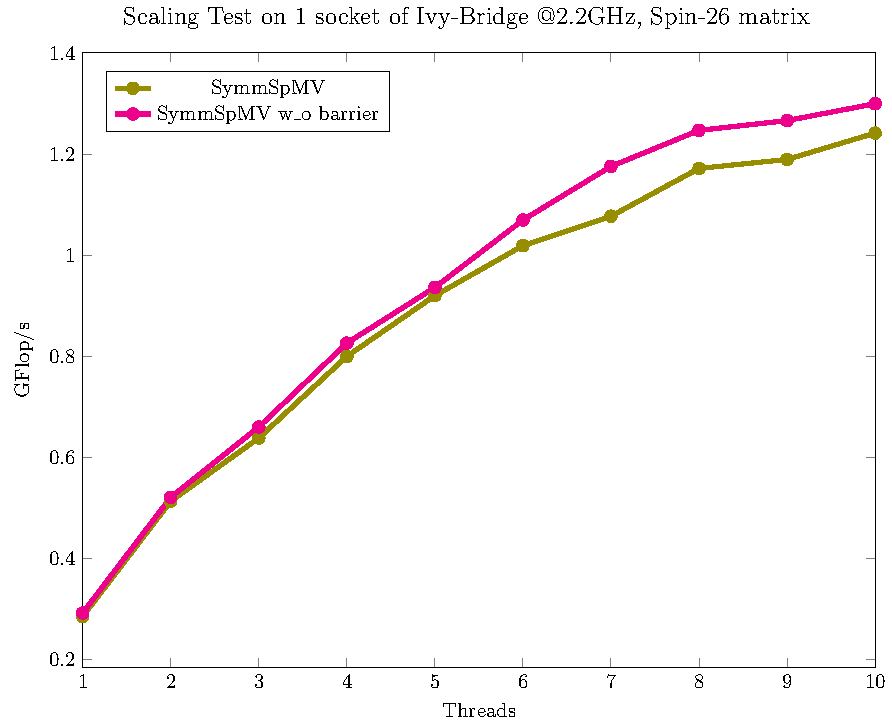
\includegraphics[width=0.45\textwidth, height=0.22\textheight]{pics/motivation/motivation_4}}
  	\caption{Effect of Multicoloring}
  	\label{fig:motivation}
  \end{figure}
  
 In order to get a better understanding of the underlying problem it's convenient to choose simple sparse matrix transpose vector (\SpMTV) as a benchmark kernel. The particular choice of this kernel is due to the fact that both \KACZ and \SpMTV have similar kind of dependencies, and it's much easier to compare with our reference kernel namely sparse matrix vector (\SpMV) which is embarrassingly parallel. The algorithm for \SpMTV and \SpMV has been listed in \cref{alg:SpMTV,alg:SpMV}
 
%  \begin{figure}[htbp]
 % 	\centering
  %	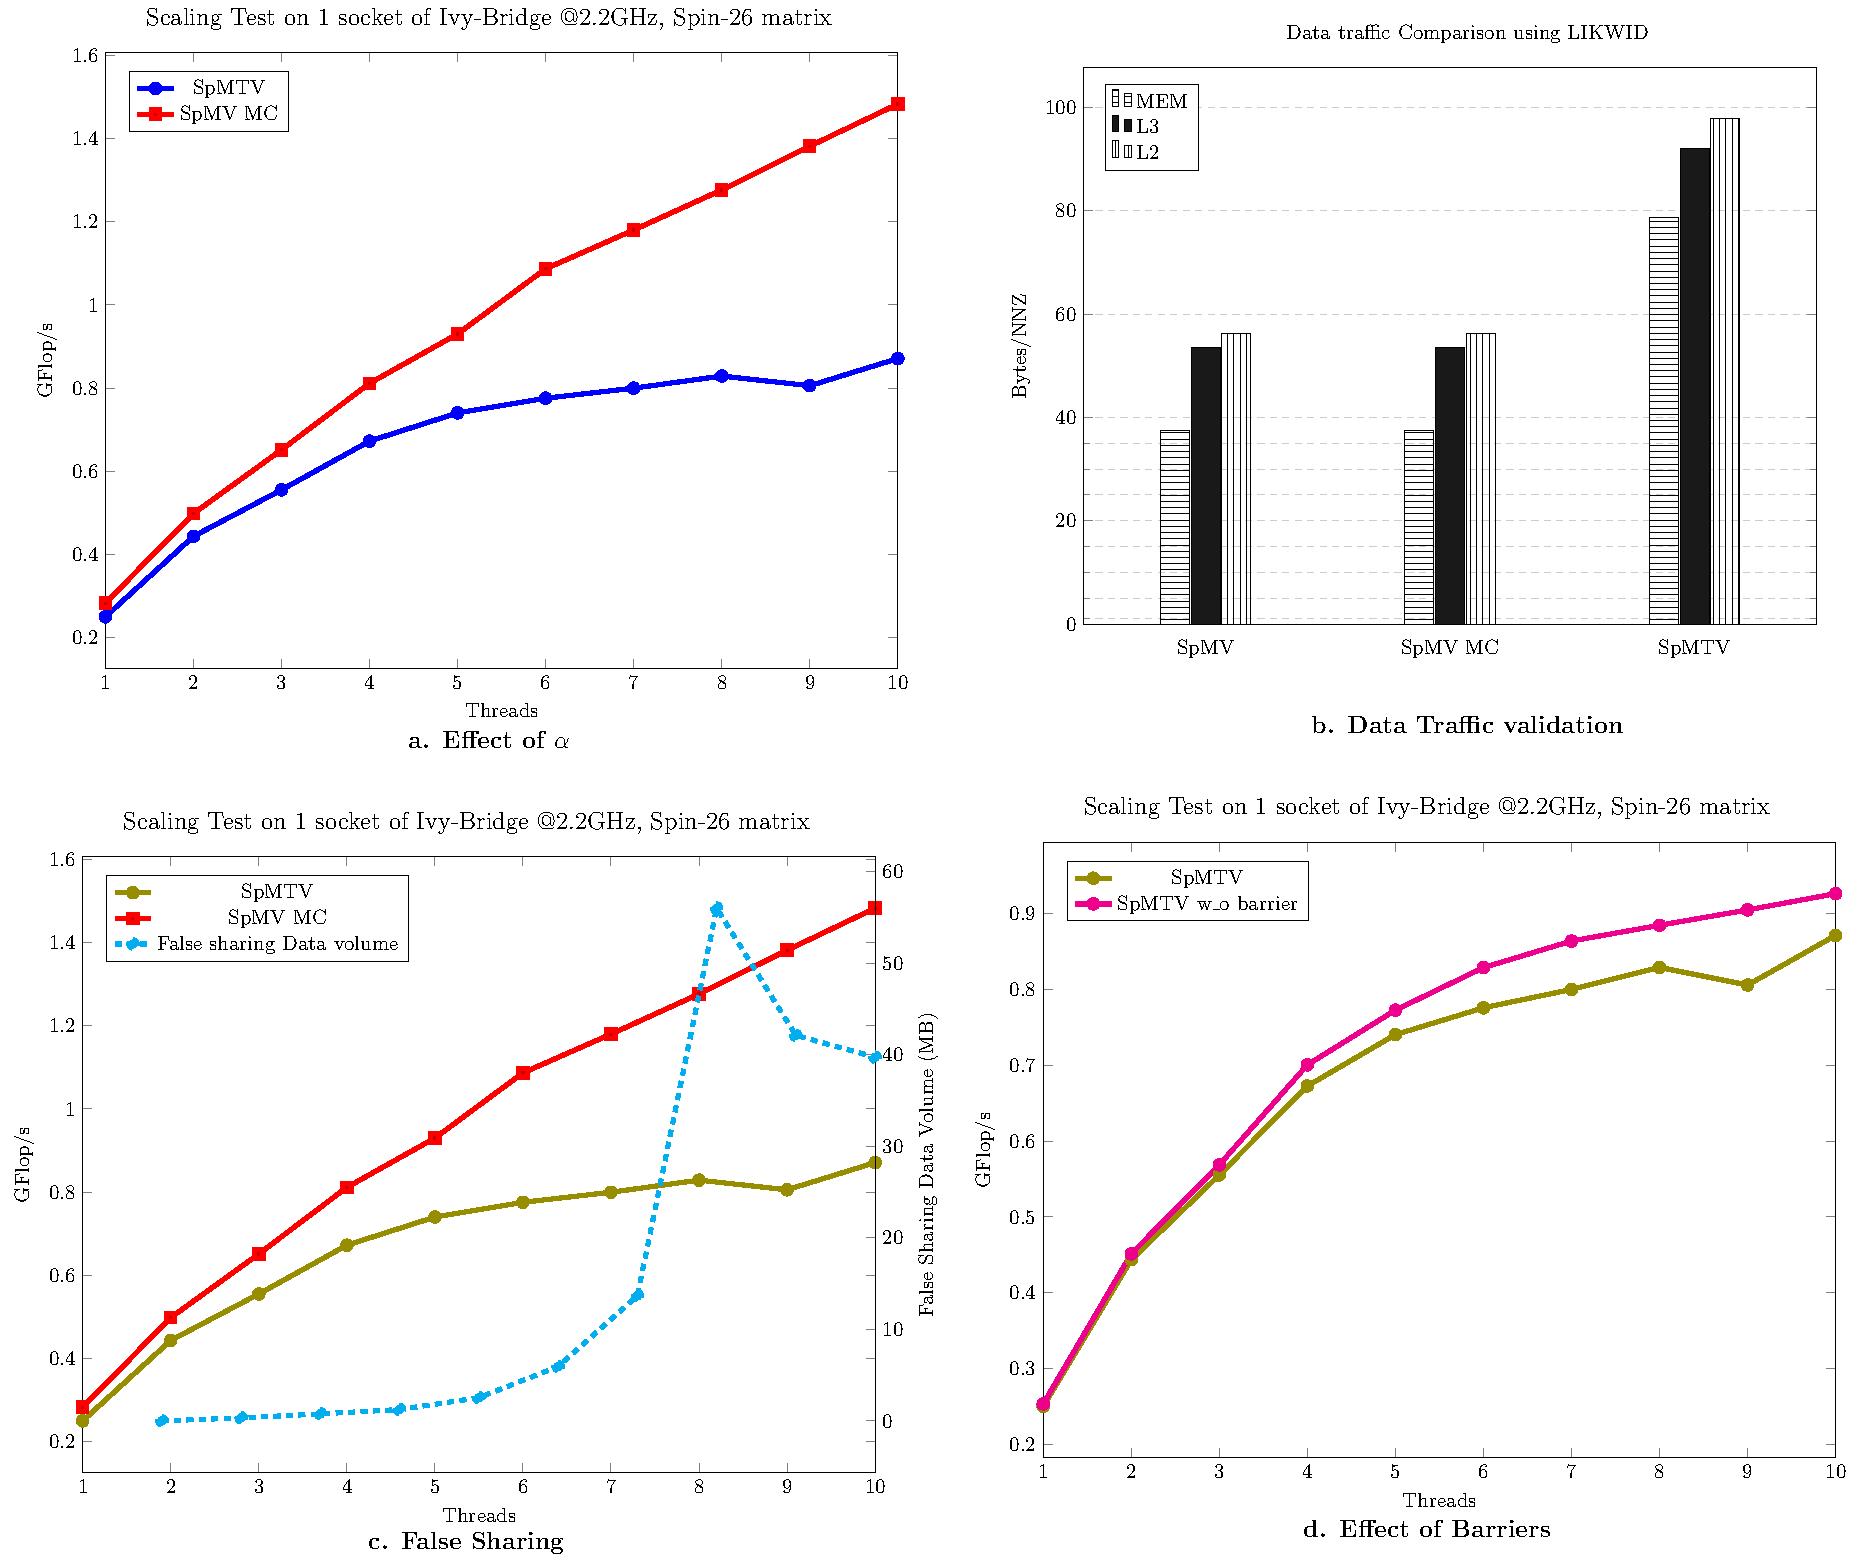
\includegraphics[width=0.9\textwidth, height=0.4\textheight]{pics/motivation/motivation}
  %	\caption{Illustration of increase in $\alpha$ by multicoloring, numbers represents thread numbers working on a particular row}
  %	\label{fig:motivation}
  %\end{figure}
 
  
 \Cref{fig:motivation_a} shows the performance of \SpMV kernel on original unpermuted matrix and matrix with \MC permutation. Here we see the performance of \SpMV on multicolored matrix is  five times  worse than that of  \SpMV on unpermuted matrix. One of the major reason for this drop is due to the increase in $\alpha$ factor seen in the intensity equation \cref{eq:SpMTV_intensity}  Since the kernels like \SpMV  are mainly memory bound increase in $\alpha$ lowers intensity $I_\mathrm{\SpMV}$ leading to a drop of performance as predicted by \roofline model \cite{Williams_roofline}. This could easily be demonstrated by measuring the data traffic between different memory hierarchies.  We do this using the \LIKWID tool \cite{LIKWID}, and the measurements can be seen in \cref{fig:motivation_b}. One can see an increase in data-traffic from all the memory hierarchy compared to \SpMV on normal unpermuted matrix. This is basically caused by the bad data locality introduced by \MCfull permutation.
 
  \begin{figure}[htbp]
  	\centering
  	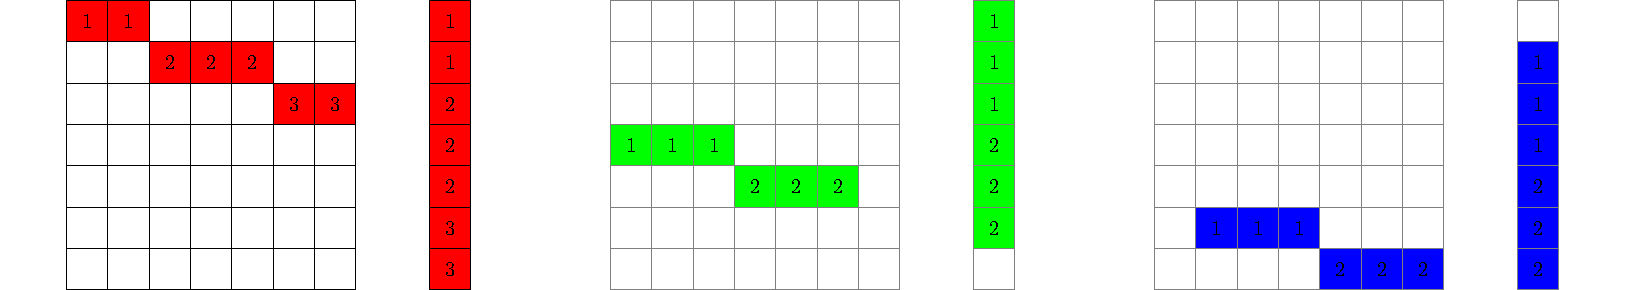
\includegraphics[scale=0.45]{pics/mc_alpha_problem/mc_alpha}
  	\caption{Illustration of increase in $\alpha$ by multicoloring, numbers represents thread numbers working on a particular row}
  	\label{fig:mc_alpha}
  \end{figure}
  
  \Cref{fig:mc_alpha}  shows an illustration of why data traffic increases for a given matrix. If one assumes last level cache (\LLC) can only hold less than six elements and obeys perfect LRU policy, as seen in the \cref{fig:mc_alpha} for  each new color we would need to load the data from main memory. As we will see later this $\alpha$ factor strongly depends on the matrix size and the size of \LLC.
  
 As seen in \cref{fig:motivation_b} the data traffic further increases for \SpMTV due to additional indirect writes (scatter) and this scales up $\alpha$ factor as seen in the denominator of $I_{\SpMTV}$ (see \cref{eq:SpMTV_intensity}),  which further decreases performance of \SpMTV compared to \SpMV on \MC matrix. 
 
 Other contributors to the drop in performance is global synchronizations and false sharing. These factors strongly depend on the number of colors and in general increase with chromatic number. For the Spin matrix the overhead of synchronization is roughly 10\%.  For most of the matrices one could also observe a strong positive correlation between false sharing and number of threads for \SpMTV kernels, due to the indirect writes in \SpMTV.

It was seen that for most of the matrices arising in the project average drop in performance by \MCfull was almost a factor of two on a single socket of \IVB. Although for most of them performance could be improved by \ABMCfull (\ABMC), still the results we obtained were not optimal (especially for large matrices) when compared to performance models which we will see later in \cref{Sec:expt}. This led to the development of a method which works on a common data format like \CRS in which most of the other kernels are written and at the same time preserves data locality, reduce synchronization overheads and false sharing.


 

